Even with significant investments in algorithm development and
selection, the computational costs of running a visual assist system
on traditional computing platforms can still be significant and a
potential impediment to practical deployment. In this section we
describe efforts to implement custom designs for assistive vision,
leverage new, non-traditional architectures, and forecast the impact
of emerging technologies that can further improve the efficiency and
effectiveness of visual assist systems from the wearable front ends
and mobile edge computing platforms through the cloud-hosted back-ends
and databases.

\subsection{Custom Chips}
While the computational needs of the computer vision algorithms we
employ are substantial, they are also heavily structured and ammenable
to acceleration. The computation and memory management for sub-tasks,
such as person-detection or recognizing sets of replicated objects on
grocery shelves, can be heavily customized to yield both large
performance and energy gains. We have developed FPGA-based solutions
for these sub-tasks, although our designs could also translate to ASIC
implementations.

In ~\cite{fpl2015}, the authors proposed a scalable solution for object 
detection using structured features - Histogram of Oriented Gradients.
While these features are very lightweight in terms of hardware resources, 
the high miss-rate is cause for concern. On the other hand, a deep CNN 
would have better accuracy, but would struggle to meet stringent power 
and area constraints when being deployed onto a wearable platform. Our 
current work is focussed on reducing the detection threshold and using 
these detection outputs as region proposals to a shallow CNN. 
Figure~\ref{fig:customchips} shows the output of our structured HOG
custom hardware alongside a combined HOG-CNN approach.

%Coupling structural with learned features
\begin{figure*}[!htb]
\centering
\begin{tabular}{@{}c@{} @{\hspace{1em}}c@{} @{\hspace{1em}}c@{} @{\hspace{1em}}c@{}}
\vspace{-5pt}
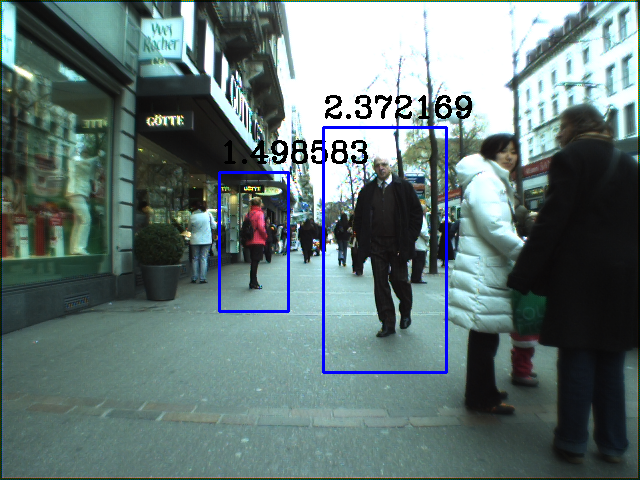
\includegraphics[width=0.22\linewidth,trim={0 0 0 0},clip]{oc_image_00000596_0.png} & 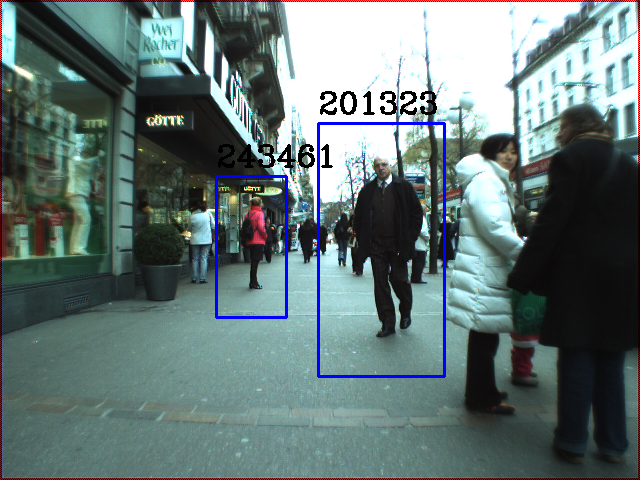
\includegraphics[width=0.22\linewidth,trim={0 0 0 0},clip]{hwpedro_122000_image_00000596_0.png} & 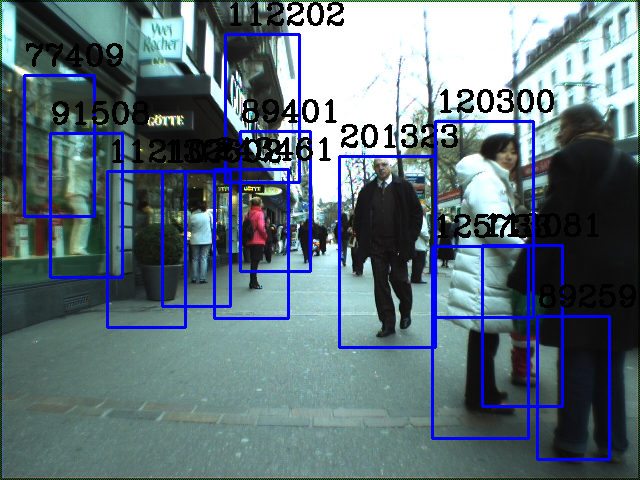
\includegraphics[width=0.22\linewidth,trim={0 0 0 0},clip]{hwpedro_61000_image_00000596_0.png} & 
\includegraphics[width=0.22\linewidth,trim={0 0 0 0},clip]{MissingFigure.pdf}\\[\abovecaptionskip]
\small(a) OpenCV output & \small (b) Hardware HOG output ~\cite{fpl2015} & \small (c) Reduced threshold & \small (d) HOG-CNN output \\
\end{tabular}
\caption{Coupling structured features with learned features}
\label{fig:customchips}
\end{figure*}

\subsection{Brain-like Architectures}
The increasing prevalence of brain-inspired algorithms, such as
saliency, and the dramatic rise in the use and utility of machine
learning workloads has inspired research into architectures that more
directly embody brain-like functionality. These new architectuures,
such as IBM's TrueNorth~\cite{truenorth} completely abandon the
traditional, centralized von-Neumann architectures of general purpose
computing for distributed, neuro-inspired computation models. While
moving tasks to these new brain-like architectures generally requires
significant rethinking and re-expression of the existing codebases,
for tasks that were already modeling neural networks, such as many
machine learning workloads, the impacts can be both rapid and
profound.

IBM's TrueNorth chip is an architypical example of this new class of
brain-like architectures. It consists of 4096 neurosynaptic cores
arranged in a 2-D array occupying 4.3 ${cm^2}$ of area in a 28~nm low
power CMOS process. A key advantage of this chip is that it consumes
merely 65~mW of power while running a typical computer vision
application~\cite{truenorth}. Having accelerated some of the key
computer vision models using custom fabrics like FPGAs and GPUs, we
are now looking to map them onto TrueNorth. While our FPGA and GPU
acceleration efforts have supported real-time performance levels and
greatly increased power efficiency over traditional software
approaches, moving to these new brain-like architectures offers the
potential to push computation even closer to the sensing platform by
easily operating within wearable power budgets. Figure~\ref{tab:tn}
shows the success of one such mapping effort, depicting the output of
the HOG-based person detection approach when modeled for TrueNorth.

%TN
\begin{figure*}[!htb]
\centering
%\def\arraystretch{1.5} %
\begin{tabular}{@{}c@{} @{\hspace{2em}}c@{} @{\hspace{2em}}c@{}}
\vspace{-5pt}
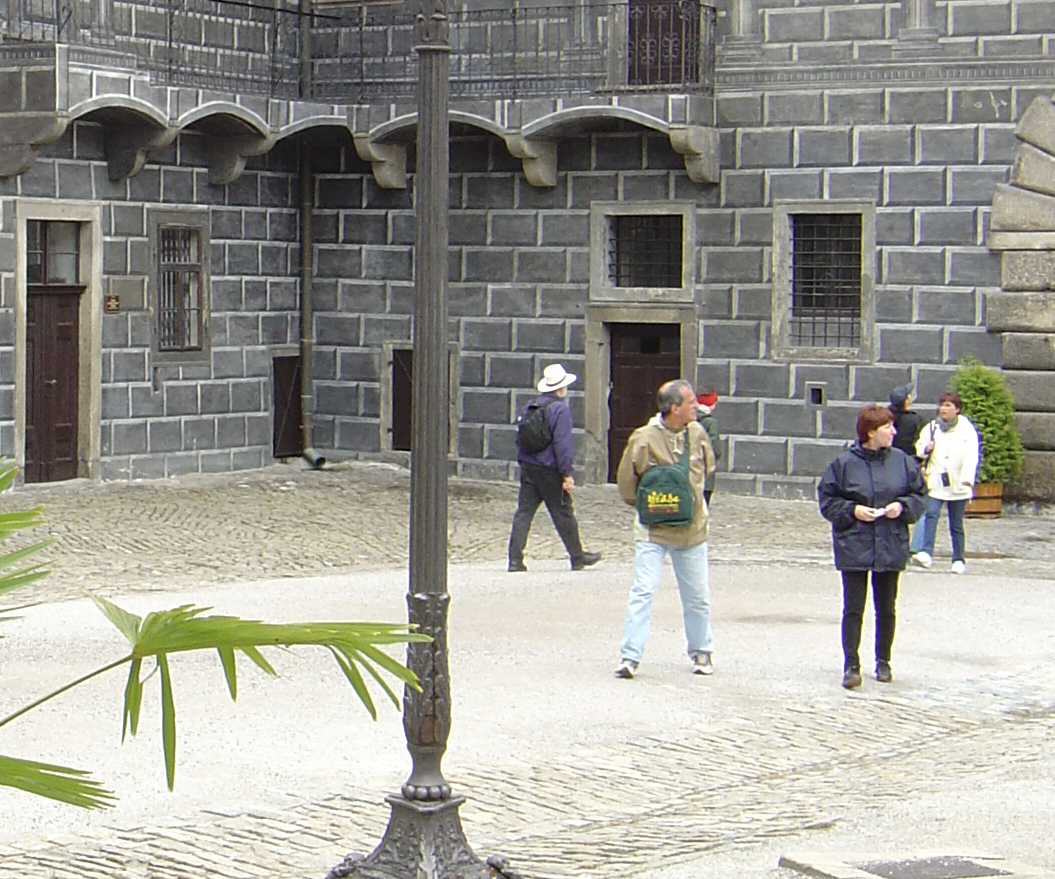
\includegraphics[width=0.29\linewidth,trim={0 0 0 0},clip]{tn_input_46.png} & 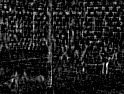
\includegraphics[width=0.32\linewidth,trim={0 0 0 0},clip]{tn_dotp_46.jpg} & 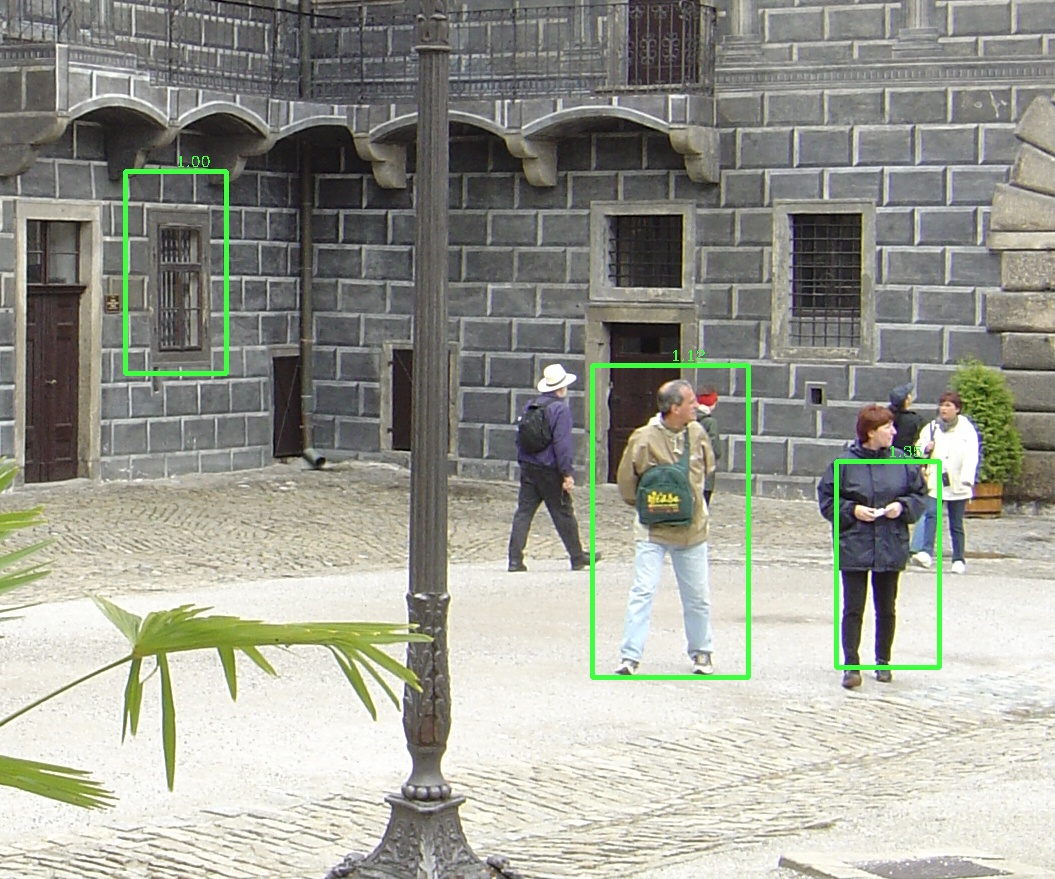
\includegraphics[width=0.29\linewidth,trim={0 0 0 0},clip]{tn_detection_46.jpg}\\[\abovecaptionskip]
\small(a) Original image & \small (b) Dot Product & \small (c) Detections \\
\end{tabular}
\caption{Mapping HOG to True North}
\label{tab:tn}
\end{figure*}

\subsection{Emerging Devices}
In addition to advances in novel architectures for vision, there are
also new emerging technologies on the horizon that can potentially
offer enable new visual computing paradigms. One such promising
technology is weakly-coupled nano-oscillators. There is an existing
body of work that shows how the analog functions of weakly-coupled
oscillators can be used to provide distance-like metrics as a new
analog primitive~\cite{upitt} and how sets of oscillators can implement
analog convolutions and other useful high-level computational
primitives. Recent advances in materials and device technologies
offers the promise of nano-scale oscillators, such as hyperFET-based
oscillators~\cite{wtsai}, that can implement these functions in extremely
small area and power budgets.

Nano-oscillators are particularly intriguing for wearable vision
applications. Early explorations indicate that arrays of
hyperFET-based oscillators are small enough and consume sufficiently
little power to be directly integrated into the image sensing
chips. In addition to the benefits from offering higher-level analog
primitives that improve computational efficiency relative over digital
calculations, recent work has highlighted the large system-level
benefits of moving early computation to the sensor chip~\cite{redeye},
thereby limiting the losses incurred in moving data from the sensing
to computing portions of wearable and mobile systems. Fully exploiting
the potential of these nano-oscillators will, however, require
substantial remapping efforts for existing computations. Our group has
mapped a number of image pre-processing primitives onto
coupled-oscillator arrays, and efforts are underway to map larger
computations, such as HOG.
